\section{引言与技术背景}
\label{sec:introduction}

\subsection{分布式 MoE 训练的通信瓶颈}

Mixture-of-Experts（MoE）通过路由器为每个 token 选择 Top-1 或 Top-2 个 expert，使模型在不按比例增加单 token 计算量的情况下扩大参数规模。在专家并行中，不同 GPU 保存不同专家；如果 token 所在 GPU 与目标专家不一致，系统就要发送 hidden state，执行专家计算，再把结果返回原来的计算流，反向阶段还需沿专家路由回传输入梯度；如存在专家副本，其参数梯度的汇总或同步取决于具体并行方案。这一前向分发、专家计算和结果回收过程通常表现为 All-to-All，而不是所有 GPU 共享同一结果的 All-Reduce。NetMoE 指出，一个 MoE 层在一次前向与反向迭代中可能涉及四次 All-to-All\cite{ref3}。

在 Scale-out 集群中，机内 NVLink、NVSwitch 或 PCIe 与跨节点链路的带宽和延迟不同，动态路由又使通信矩阵随输入变化。token 访问远端专家时可能产生跨节点传输等待，热门专家可能引起计算排队；专家容量受限时还可能造成 Token Dropping。Janus 在 16 与 32 张 A100 的多组 MoE 训练实验中报告，All-to-All 通信时间占单次迭代时间的 38.5\%--68.4\%\cite{ref1}。因此训练延迟并非显卡矩阵乘法时间的简单总和，通信路径和专家负载都可能成为瓶颈。

\subsection{静态专家放置的局限性}

固定专家、移动 token 会同时暴露两类压力：位置不匹配造成跨节点搬运，热门专家可能排队，容量受限还会造成 token dropping。扩大容量可以减少 token 丢弃，却可能增加填充和无效计算；提高负载均衡辅助损失项的权重虽能改善负载，也可能改变专家专门化。FlexMoE 的 Swin-MoE 例子显示，负载均衡辅助损失项的系数（balance loss coefficient）从 0 调至 0.05 时，GPU 利用率由 18.77\% 提升到 63.30\%，Top-5 准确率由 94.588\% 变为 93.981\%\cite{ref2}。

增加网络带宽只能直接缓解传输，路由平衡也不能保证 token 已经靠近目标专家。静态布局没有根据路由局部性和专家热度变化重新安排数据与计算位置，而不仅是网络带宽不足，这构成了研究动态放置机制的动机。

\subsection{动态放置机制与性能影响因素}

Janus 按需拉取专家权重改变通信对象；FlexMoE、SYMI 调整专家实例数量或位置缓解负载；NetMoE 利用同一样本中 token 的路由偏好，调整样本节点与设备归属，利用机内外通信差异。这些策略受状态同步、权重搬运、映射维护、求解、显存和计算通信重叠成本约束。

核心问题是：在不同的局部性、专家热点和调整窗口下，专家拉取、专家复制与样本放置分别解决什么关键路径瓶颈，哪一种动作更可能获得端到端净收益？第 2 章比较代表性工作，第 3 章提炼未解决的矛盾，第 4 章提出个人研究思路及验证方法。图~\ref{fig:overview} 概览分布式 MoE 训练中的系统组成、静态放置挑战和动态放置主线。

\begin{figure}[!htbp]
\centering
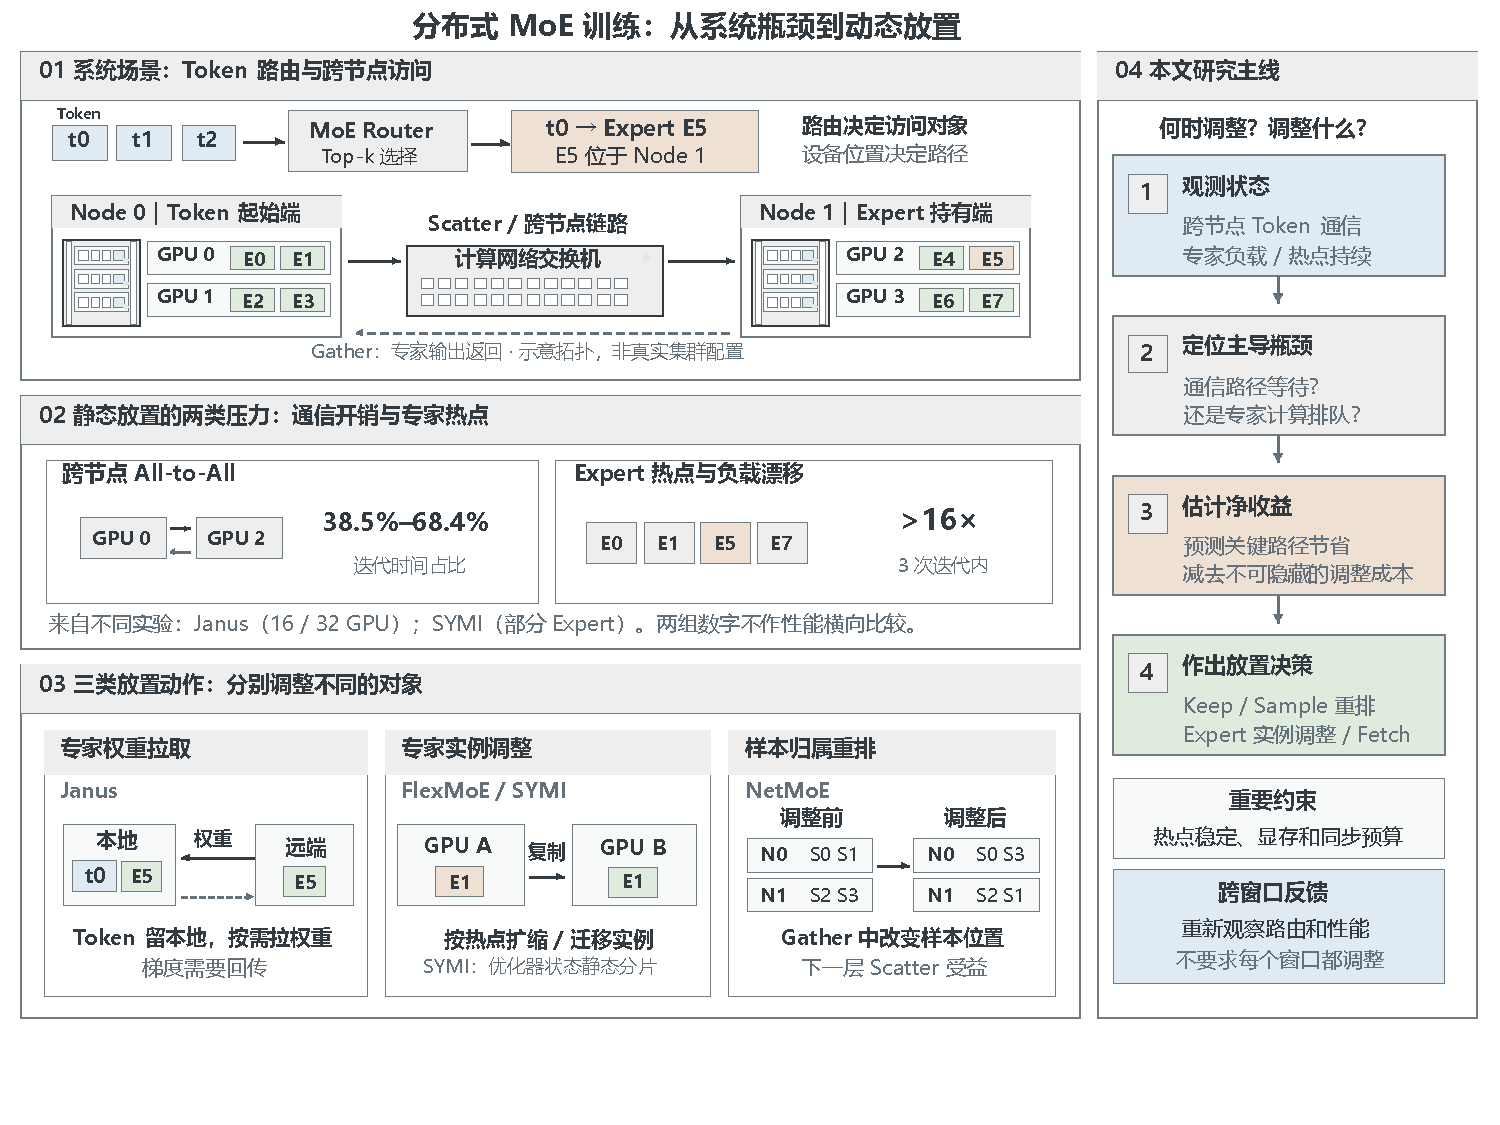
\includegraphics[width=\linewidth,trim=0 46pt 0 0,clip]{figures/figure1.pdf}
\caption{分布式 MoE 训练系统与动态放置研究主线。面板 01 为拓扑示意，面板 04 为研究设想；面板 02 的数字不作同配置比较。根据 Janus\cite{ref1}、NetMoE\cite{ref3}、SYMI\cite{ref4} 等文献整理绘制。}
\label{fig:overview}
\end{figure}

